Calcule el volumen encerrado entre el paraboloide
\[
z=4-x^2-y^2
\]
y el plano $z=1$.

\begin{center}
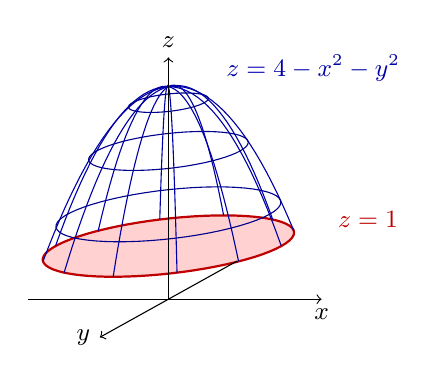
\begin{tikzpicture}[x={(0.92cm,0cm)}, y={(-0.45cm,-0.25cm)}, z={(0cm,0.75cm)}, scale=0.9, every node/.style={font=\small}]
    % Plano z=1 y su circunferencia de intersección con el paraboloide.
    \fill[red!18] plot[domain=0:360, samples=70] ({1.732*cos(\x)},{1.732*sin(\x)},1) -- cycle;
    \draw[red!75!black, thick] plot[domain=0:360, samples=70] ({1.732*cos(\x)},{1.732*sin(\x)},1);

    % Malla del paraboloide z=4-r^2.
    \foreach \angle in {0,30,...,330} {
        \draw[blue!65!black] plot[domain=0:1.732, samples=24]
            ({\x*cos(\angle)},{\x*sin(\angle)},{4-\x*\x});
    }
    \foreach \radius in {0.55,1.10,1.55} {
        \draw[blue!55!black] plot[domain=0:360, samples=60]
            ({\radius*cos(\x)},{\radius*sin(\x)},{4-\radius*\radius});
    }
    \draw[->] (-2.15,0,0) -- (2.35,0,0) node[below] {$x$};
    \draw[->] (0,-2.15,0) -- (0,2.15,0) node[left] {$y$};
    \draw[->] (0,0,0) -- (0,0,4.55) node[above] {$z$};
    \node[blue!65!black] at (2,-0.45,4.2) {$z=4-x^2-y^2$};
    \node[red!75!black] at (2.5,-1.15,1.12) {$z=1$};
\end{tikzpicture}
\end{center}
